\chapter{CUDAmino}
\label{sec:cudamino}

\chaptertoc{}

\begin{chapterabstract}
  This chapter introduces CUDAmino, a \ac{GPU} accelerated \ac{dMRI} simulator based on the \ac{MC} simulator that is part of the Camino software package \cite{Cook2006,Hall2009}.
  The main differences between CUDAmino and Camino are outlined as well as presenting some experiments assessing the performance of CUDAmino relative to Camino.
\end{chapterabstract}


\section{CUDAmino Design}
\label{sec:cudamino_design}
The basic \acl{MC} \ac{dMRI} simulation algorithm outlined in \Cref{alg:MC_random_walk} does not change when adapting the simulations to run on the \ac{GPU}, however some changes are necessary to make the simulations efficient for the \ac{GPU}.

CUDAmino is, of course, designed to exploit the parallel nature of the \ac{GPU}.
Since each spin is simulated independently of all of the other spins, the problem is inherently parallel and we can use each execution thread to simulate a single spin.

The problem could also be parallelised along the time dimension, however that can lead to a problem known as a race condition.
A race condition occurs when the program tries to do two things at once, but one should rely on the other so they must be done in order.
In this instance, you could get one thread trying to take the $(t+1)^{\mathrm{th}}$ step before the $t^{\mathrm{th}}$ step is finished.
For this reason, CUDAmino is only parallelised along the number of spins.

Another potential pitfall of GPU simulations, mentioned in \Cref{sec:bg_gpu}, is thread divergence.
In particular, the while loop in \Cref{alg:MC_random_walk} could be a source of thread divergence.
Different threads will have spins in different locations, so may end up with different numbers of iterations of the loop to amend the step.
The impact of this will be accentuated by meshes with small structures where faces are close to each other, so there may be many multiple reflections.

In order to try and minimise thread divergence, CUDAmino follows the technique of Waudby and Christodoulou \cite{Waudby2011} who use rejection sampling.
The rejection sampling technique simply checks whether any given step has crossed a face and if it has, then the step is rejected and the spin does not move.
Provided the steps are small relative to the size of the structures in the substrate, the difference between rejection sampling and reflection is minimal \cite{Johannesson1996}.

Another consideration when designing CUDAmino, was to limit the number of unnecessary collision checks.
A complex mesh may have hundreds of thousands or millions of faces, if each step in the simulation has to check all faces, it will be unnecessarily slow.
The step should, ideally, only check for collisions with those faces which are nearby to it, in doing so it may be possible to reduce the number of collision checks from hundreds of thousand to a few tens of faces.

This problem of reducing the number of faces required for collision checks is a well studied problem in the field of ray-traced graphics rendering.
A number of spatial partitioning schemes have been developed to accelerate collision checks  such as the simple uniform grid \cite{Fujimoto1986,Amanatides1987}, octree \cite{Fujimoto1986} and \ac{BVH}\cite{Kay1986}. 

So far, aligning with the \ac{CPU} Camino implementation, CUDAmino uses a simple uniform grid acceleration scheme. In short, this uniformly subdivides the space in which the mesh sits, meaning that each step need only check collisions for the triangles within the subspace that the step goes through.

\begin{figure}[t]
  \centering
  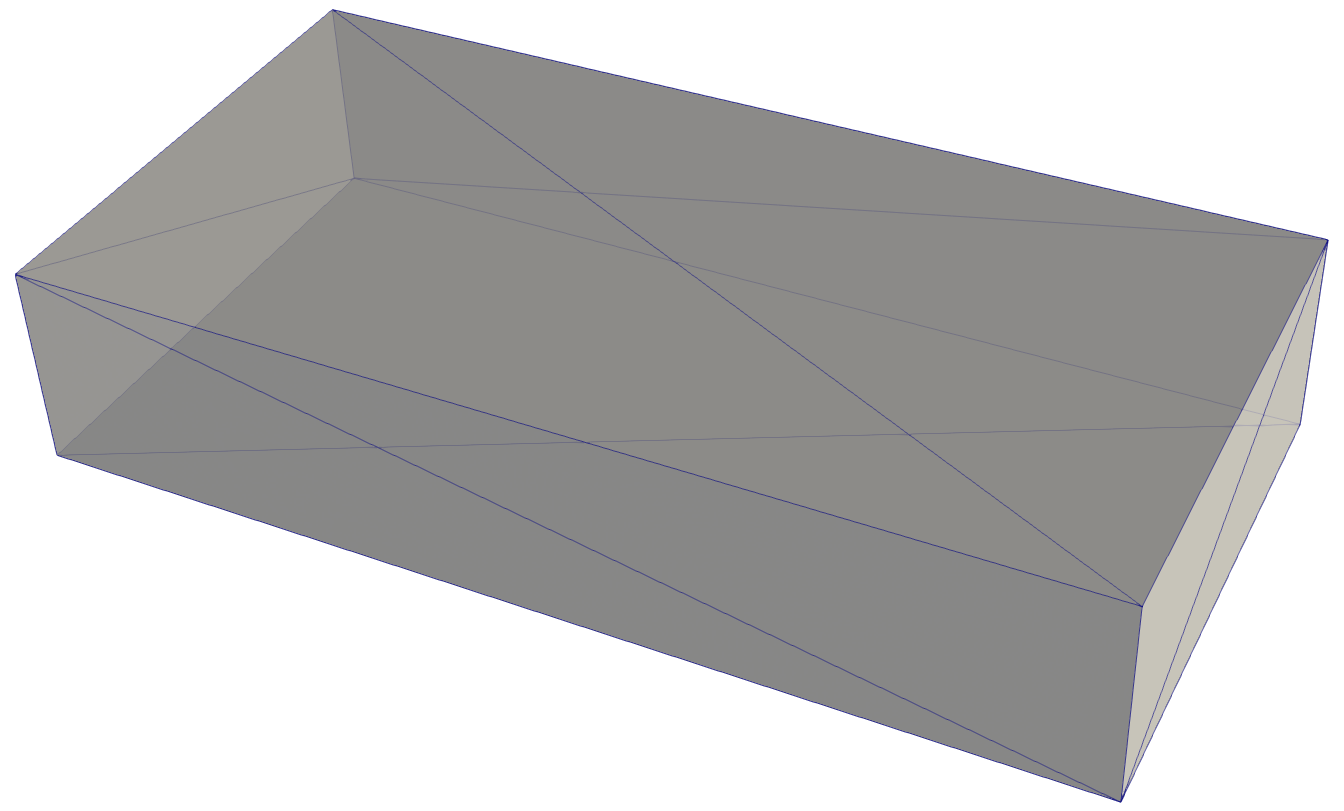
\includegraphics[width=0.7\textwidth]{figures/cudamino/cuboid_lores.png}
  \caption[Simple lo-res cuboid used for testing CUDAmino.]{Simple lo-res cuboid used for testing CUDAmino. Cuboid dimensions are $2\,\mu$m$\times5\,\mu$m$\times10\,\mu$m and it has 12 triangular faces.}
  \label{fig:cudamino_cuboid}
\end{figure}

\section{CUDAmino Experiments}
\label{sec:cudamino_experiments}
In order to test CUDAmino's performance against Camino, two experiments were carried out.
Both experiments were carried out using a simple cuboid mesh as shown in \Cref{fig:cudamino_cuboid}, which has dimensions $2\,\mu$m$\times5\,\mu$m$\times10\,\mu$m and 12 faces.
This simple substrate was chosen since the analytic solution for diffusion between two planes with a separation, $a$, is well known \cite{Callaghan1995,Linse1995}.

The first experiment investigated the effect of the number of timesteps on the resulting simulated signal.
As the number of timesteps increases, the step length decreases and the rejection sampling approach of CUDAmino should approach the reflection approach of Camino.

Simulations were run in both Camino and CUDAmino with $n = 100000$ spins and $t_{max} = 1000, 10000, 50000$ and impermeable membranes. Each experiment was repeated 5 times. 
Simulated \ac{dMRI} signals were generated using a standard \ac{PGSE} sequence with $\Delta = 50$ ms, $\delta = 0.1$ ms (very small $\delta$ to approximate \ac{SGP} regime) and $b$-value ranging from 0 to 60 ms/$\mu$m$^2$.
CUDAmino experiments are run on an NVIDIA TITAN Xp \ac{GPU} and Camino experiments are run on a 3.1GHz Intel Core i7 \ac{CPU}. 


% \begin{figure}
%   \centering
%   \begin{subfigure}{0.49\textwidth}
%     \centering
%     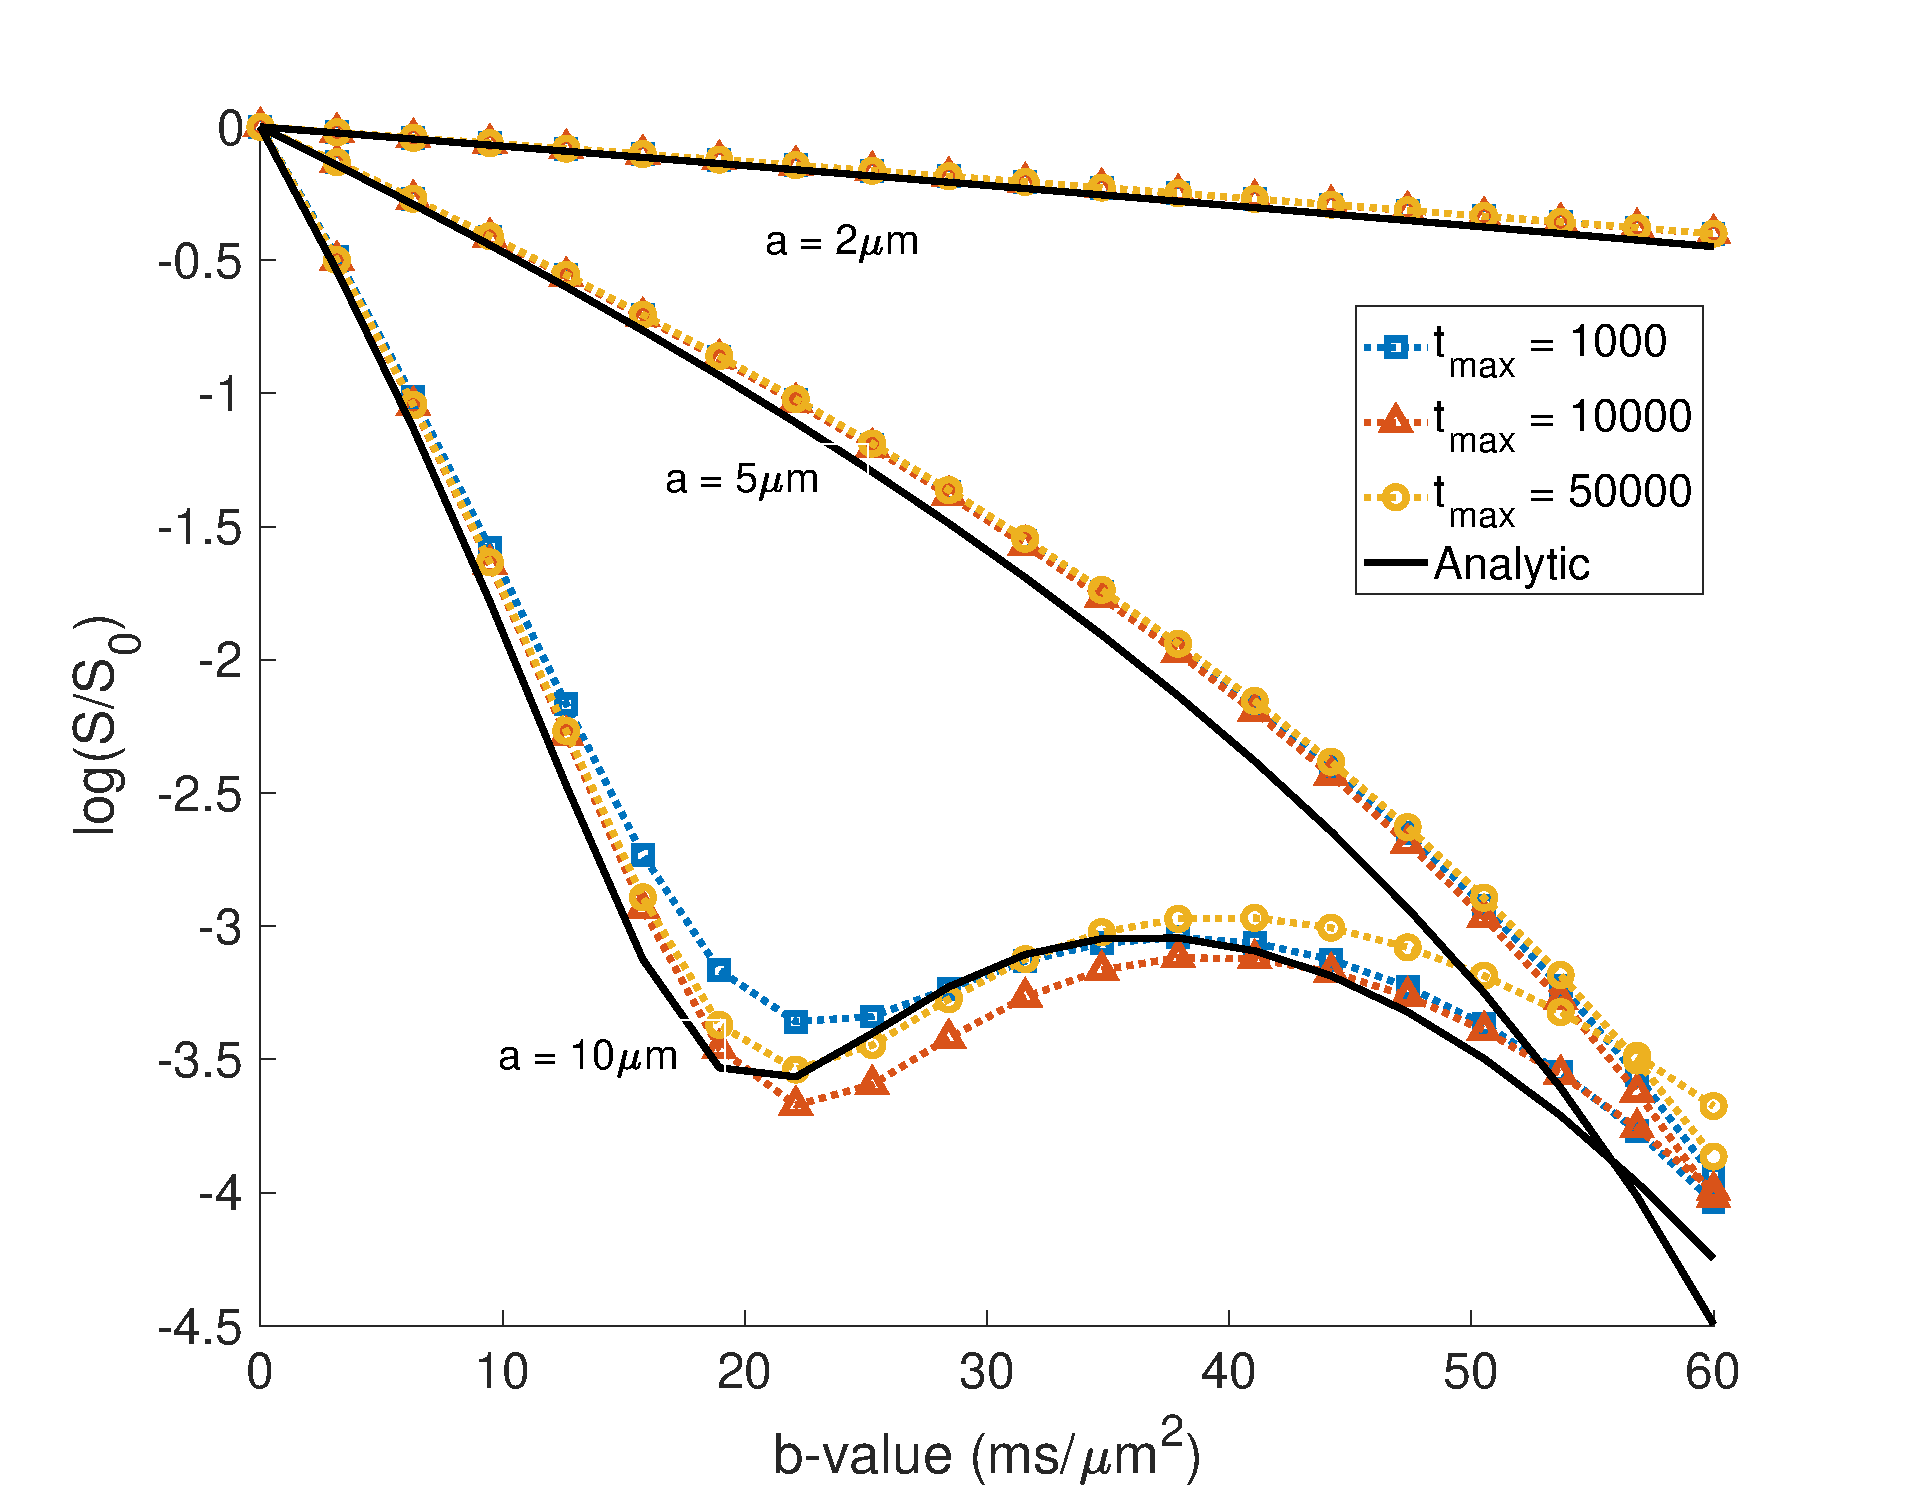
\includegraphics[width=\textwidth]{figures/cudamino/new/cuboid_all_cudamino_tmax.eps}
%     \caption{}
%     \label{fig:cyl_tmax_sig}
%   \end{subfigure}
%   ~
%   \begin{subfigure}{0.49\textwidth}
%     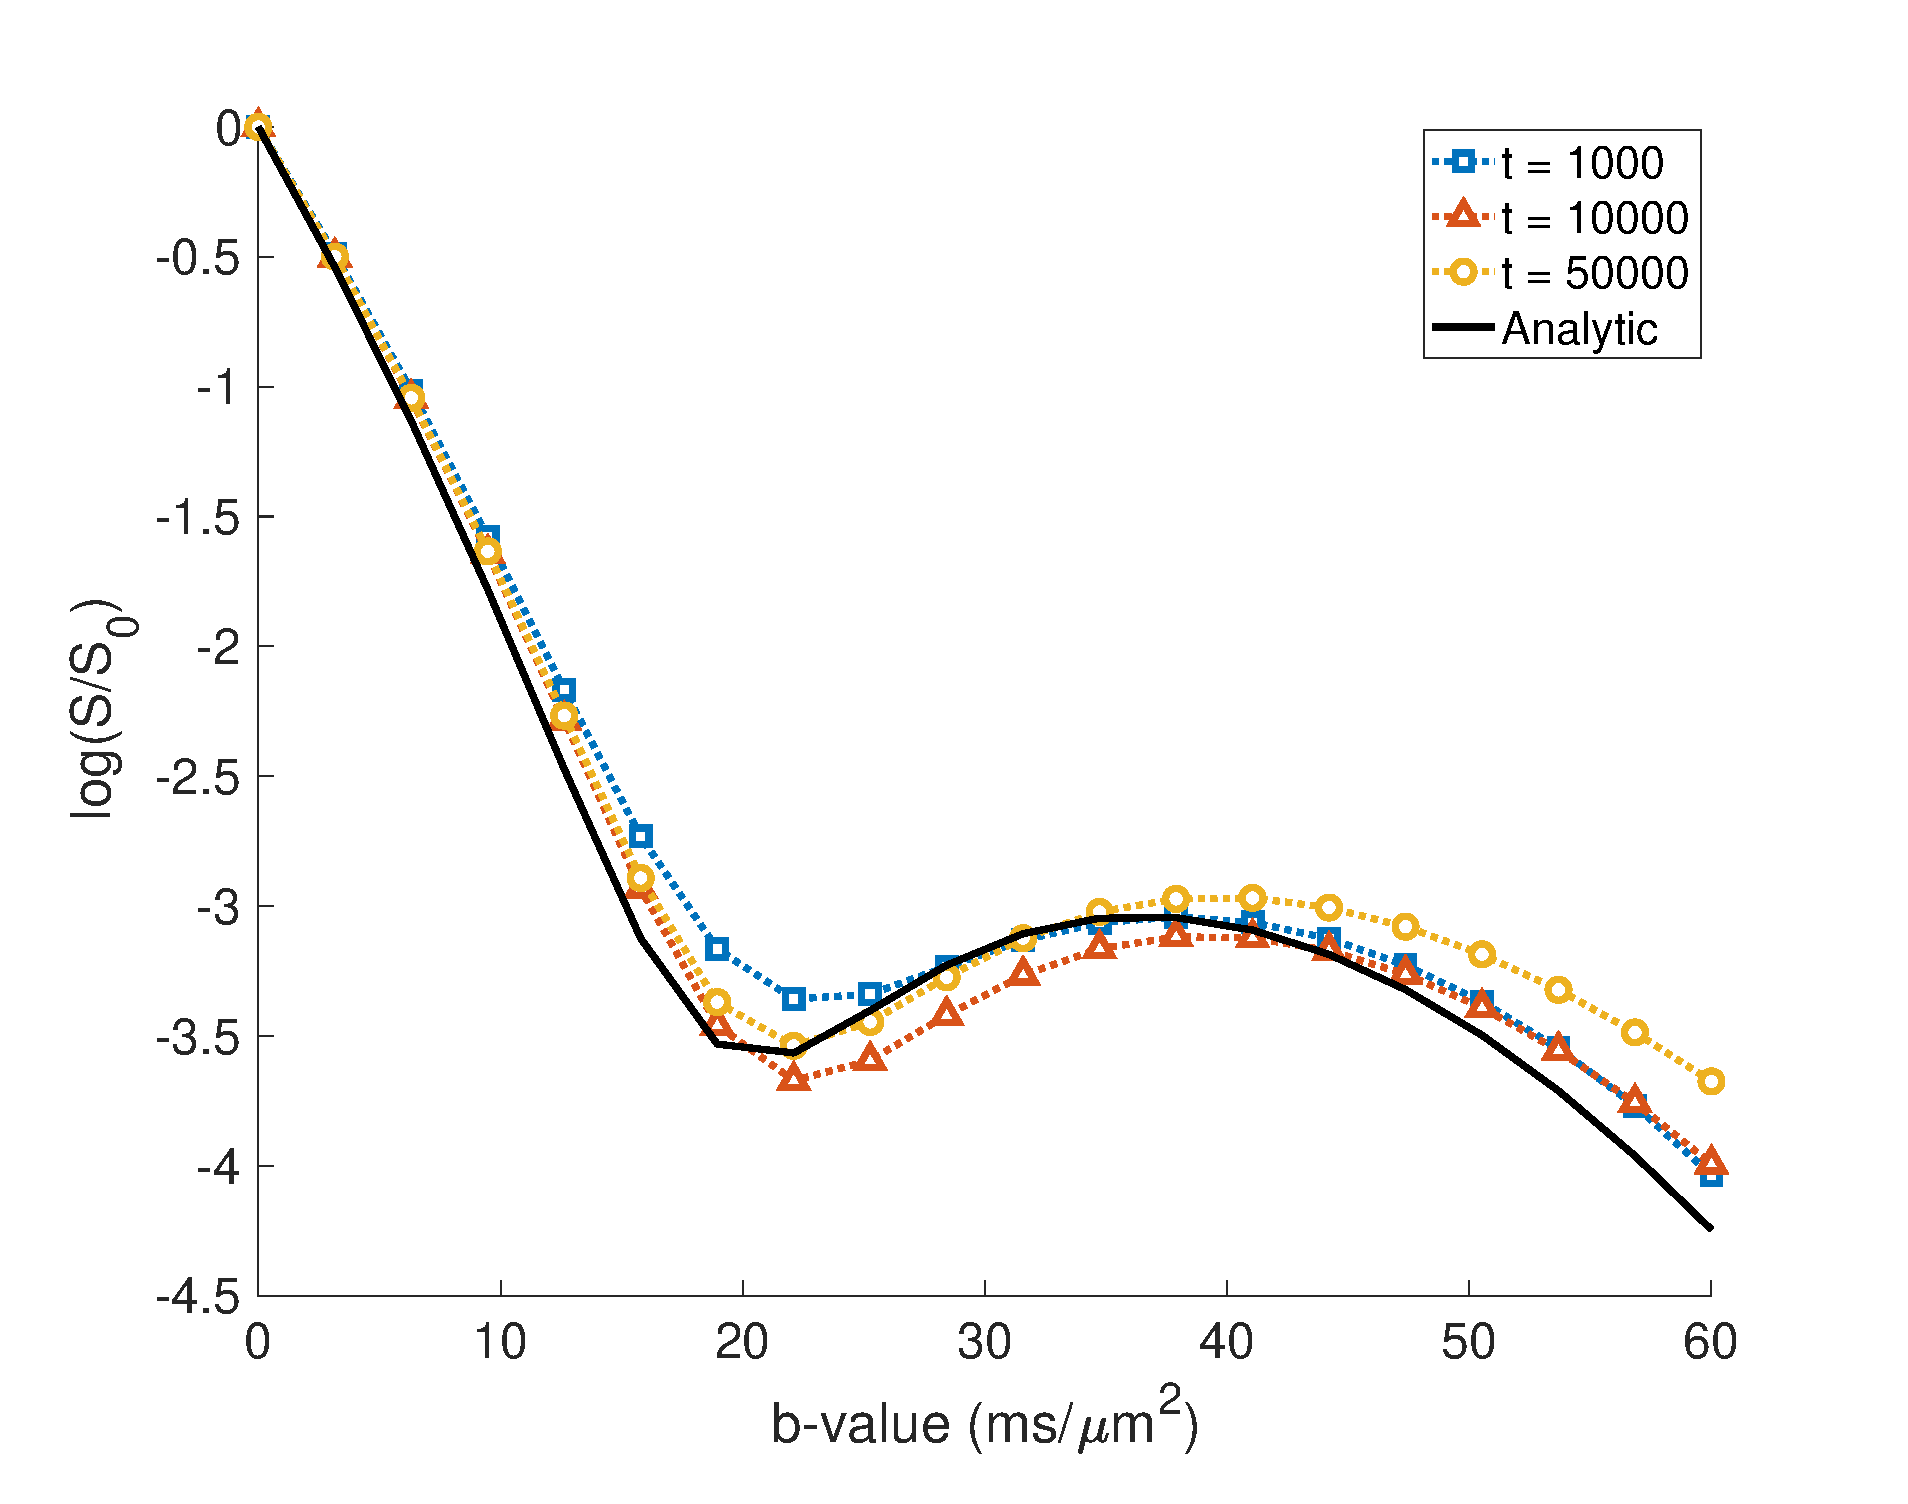
\includegraphics[width=\textwidth]{figures/cudamino/new/cudamino_10um_tmax.eps}
%     \caption{}
%     \label{fig:cyl_tmax_diff}
%   \end{subfigure}
%   \caption{Cylinder tests varying $t_{max}$. a) The simulated \ac{dMRI} signals and b) The difference between CUDAmino and Camino signals.Cylinder tmax tests}
%   \label{fig:cyl_tmax}
% \end{figure}

\begin{figure}
  \centering
  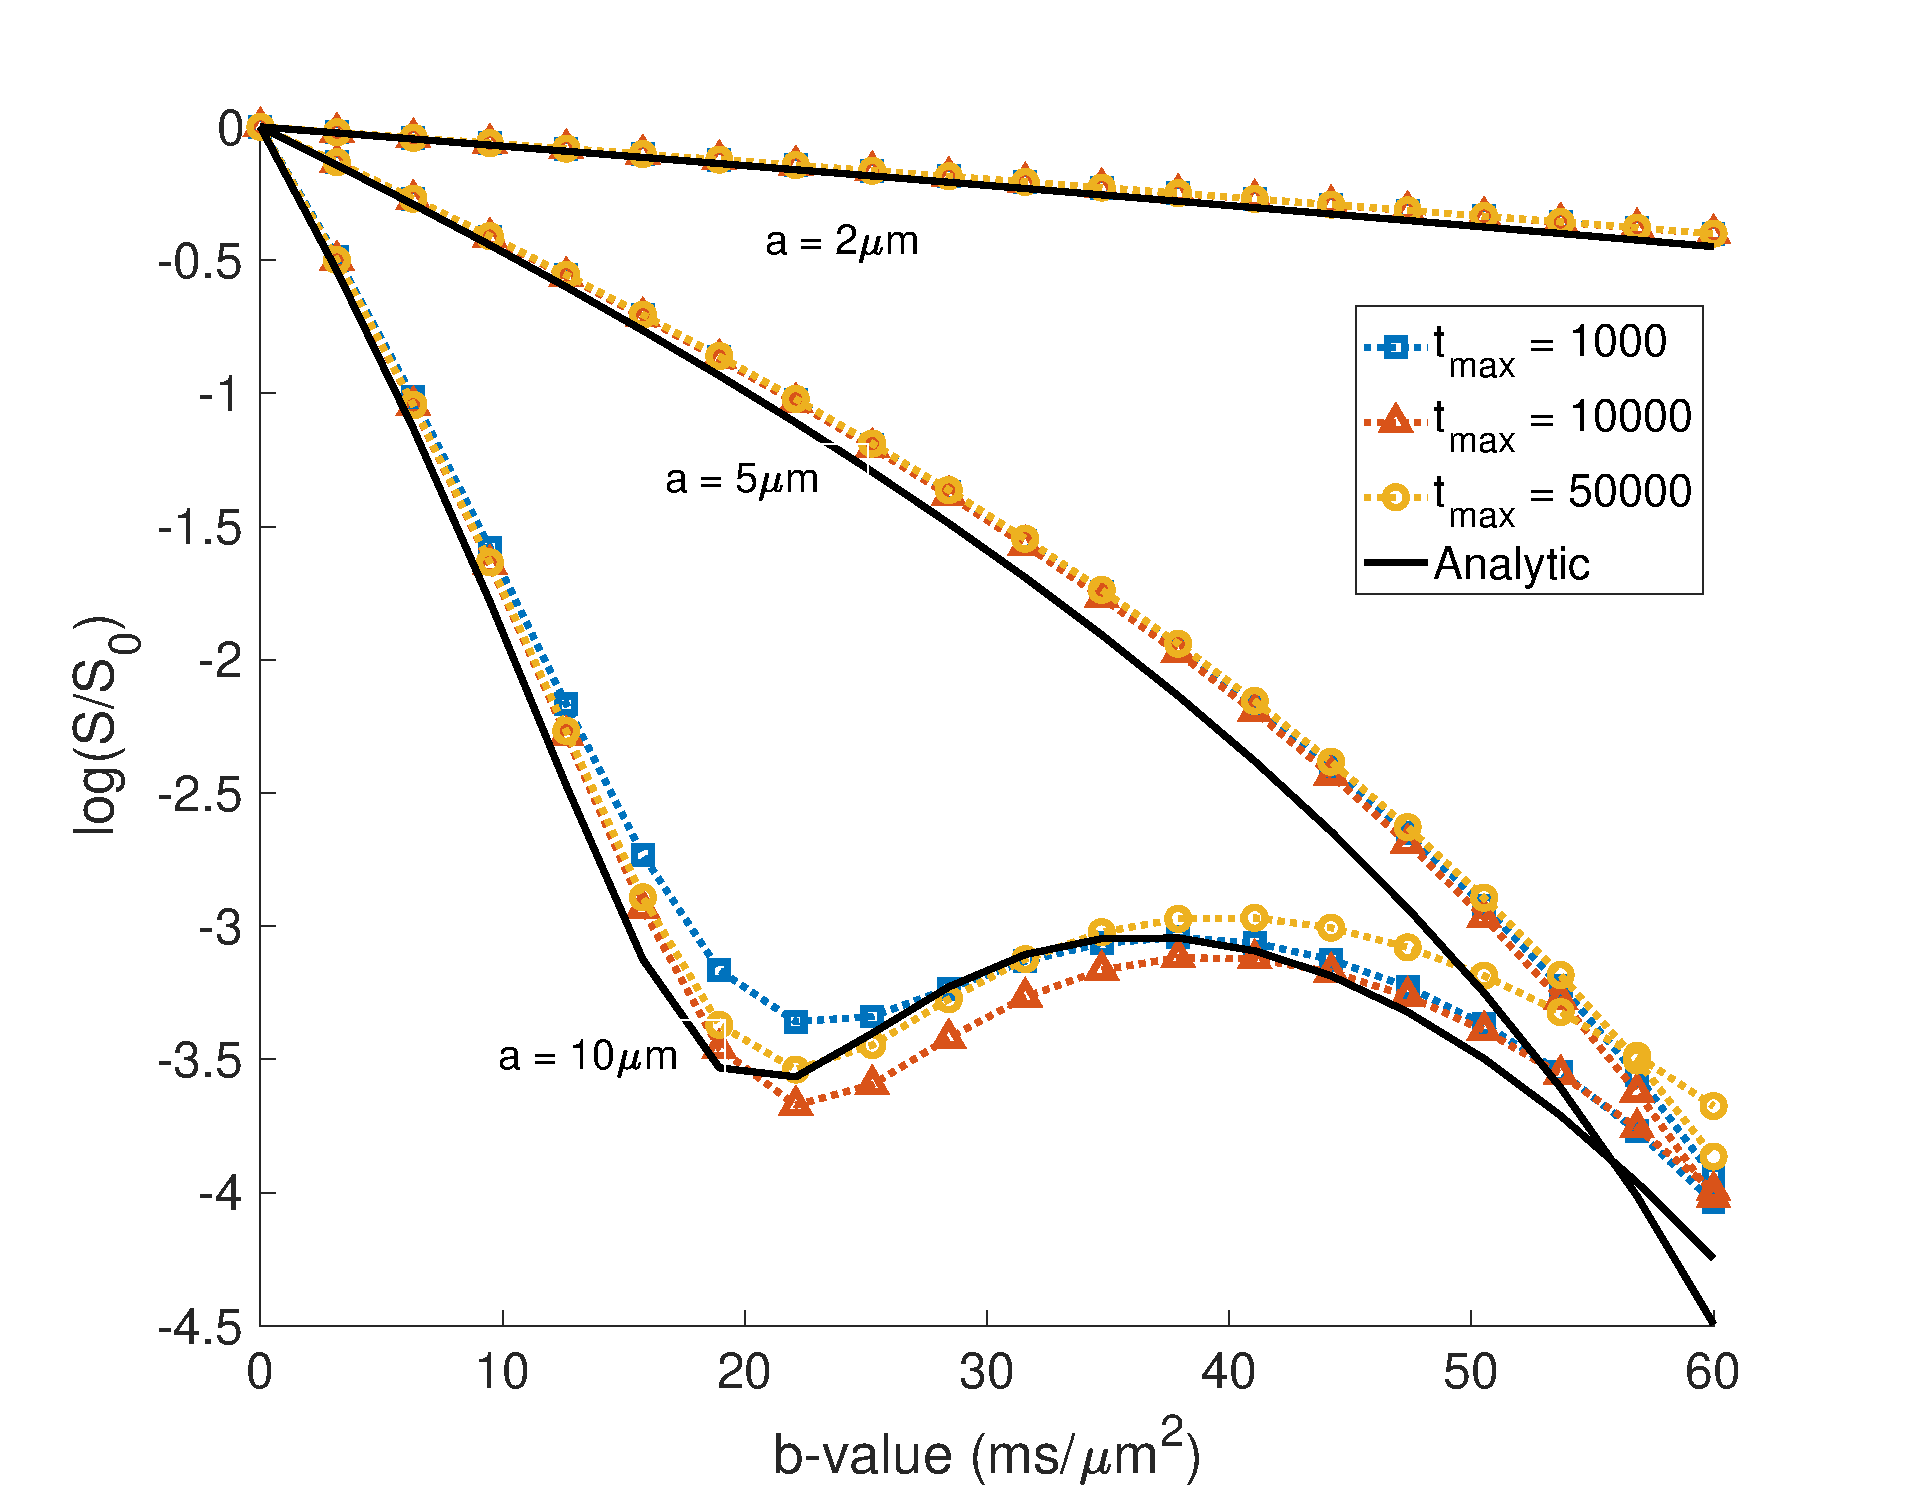
\includegraphics[width=0.8\textwidth]{figures/cudamino/new/cuboid_all_cudamino_tmax.eps}
  \caption[CUDAmino simulations versus analytic solutions for varying $t_{max}$.]{CUDAmino simulations (dotted lines) versus analytic solutions (solid black lines) for diffusion in the three directions normal to faces of the cuboid in \Cref{fig:cudamino_cuboid}. $a$ is the separation between the faces in each direction. The simulated signals match the analytic signal well, with more deviation at higher $b$-value in general. }
  \label{fig:cuboid_cudamino_tmax}
\end{figure}

% \Cref{fig:cyl_tmax} shows the results of the tests varying the number of timesteps. \Cref{fig:cyl_tmax_sig} shows the simulated \ac{dMRI} signal for both CUDAmino and Camino, while \Cref{fig:cyl_tmax_diff} shows the relative difference between the CUDAmino and Camino signals.
% The difference between the simulated signals is smallest with the highest number of timesteps, though the difference between the CUDAmino and Camino is small relative to the $S_0$ signal for all timesteps. 

\Cref{fig:cuboid_cudamino_tmax} shows the results of the tests varying the number of timesteps for CUDAmino against the analytic solution for each direction normal to the planes of the cuboid. Here $a$ is the separation between the planes. In general, CUDAmino matches the the analytic signal, with slightly more deviation from the analytic solution at higher $b$-value.
Whilst \Cref{fig:cuboid_cudamino_tmax} gives the impression that the error is highest for the largest separation, $a=10\,\mu$m, this is in part a consequence of the logarithm on the y-axis.

\Cref{tab:cuboid_results} shows the mean error between both the CUDAmino and Camino signals and the analytic solution for each value of $t_{max}$. This shows that the mean error is of a similar order for all three values of $a$. In general, the error reduces with higher $t_{max}$, though this is not the case for $a=2\,\mu m$. Additionally, the errors are similar for both CUDAmino and Camino, suggesting that the difference between the rejection sampling and reflection approaches is minimal, at least for this simple substrate. 

A similar experiment was carried out, varying the number of spins rather than the number of timesteps.
In this case, $t_{max}$ was fixed to 5000 and $n = 1000, 10000, 100000$.
The same \ac{PGSE} sequence parameters were used.

\Cref{fig:cuboid_cudamino_nspin} shows the results of the tests varying $n$ for CUDAmino against the analytic solutions. Again, the simulations generally match the analytic solutions well, with higher $n$ matching more closely as would be expected. As in the $t_{max}$ varying case, the deviation from the analytic solution tends to increase with increased $b$-value.

Again, \Cref{tab:cuboid_results} shows the mean error between both the CUDAmino and Camino signals and the analytic solution.
Similarly to the varying $t_{max}$ case, the error is comparable between CUDAmino and Camino and for both tends to decrease slightly  with increasing $n$. 

The main reason to develop CUDAmino for the \ac{GPU} was to speed up the simulations by exploiting the parallelism on the \ac{GPU}.
To test the speedup achieved, each simulation was timed.
\Cref{tab:cuboid_timing} shows the results of timing the CUDAmino and Camino simulations.
CUDAmino achieves a shorter running time in each case, with most simulations having a  $100\times$ speedup compared to Camino.
The one case in which CUDAmino does not achieve a $100\times$ speedup is the $n=1000$ case in which it has a $15\times$ speedup.
This is likely due to $n=1000$ not being enough spins to fully exploit the parallelism of the GPU and being limited by overheads such as copying data from the \ac{CPU} to \ac{GPU}.


% \Cref{fig:cyl_nspin} shows the results of the simulations with different numbers of spins. \Cref{fig:cyl_nspin_sig} shows the simulated signal for both CUDAmino and Camino.
% \Cref{fig:cyl_nspin_diff} shows the difference between CUDAmino and Camino. In this case, an increased number of spins increases the difference between the simulated signals.
% This suggest some systematic difference between CUDAmino and Camino which is greater with larger numbers of spins.
% This could be due to the differences between rejection sampling and reflection building up more and more with increased numbers of spins, however this requires further investigation.

% \Cref{tab:cyl_tmax_time,tab:cyl_nspin_time} show the differences in running time between Camino and CUDAmino for both experiments.
% In both cases, CUDAmino executes significantly faster, with 60-100$\times$ speedup in the $t_{max}$ case and a best case improvement of 15$\times$ for the $n$ test.




% \begin{figure}
%   \centering
%   \begin{subfigure}{0.49\textwidth}
%     \centering
%     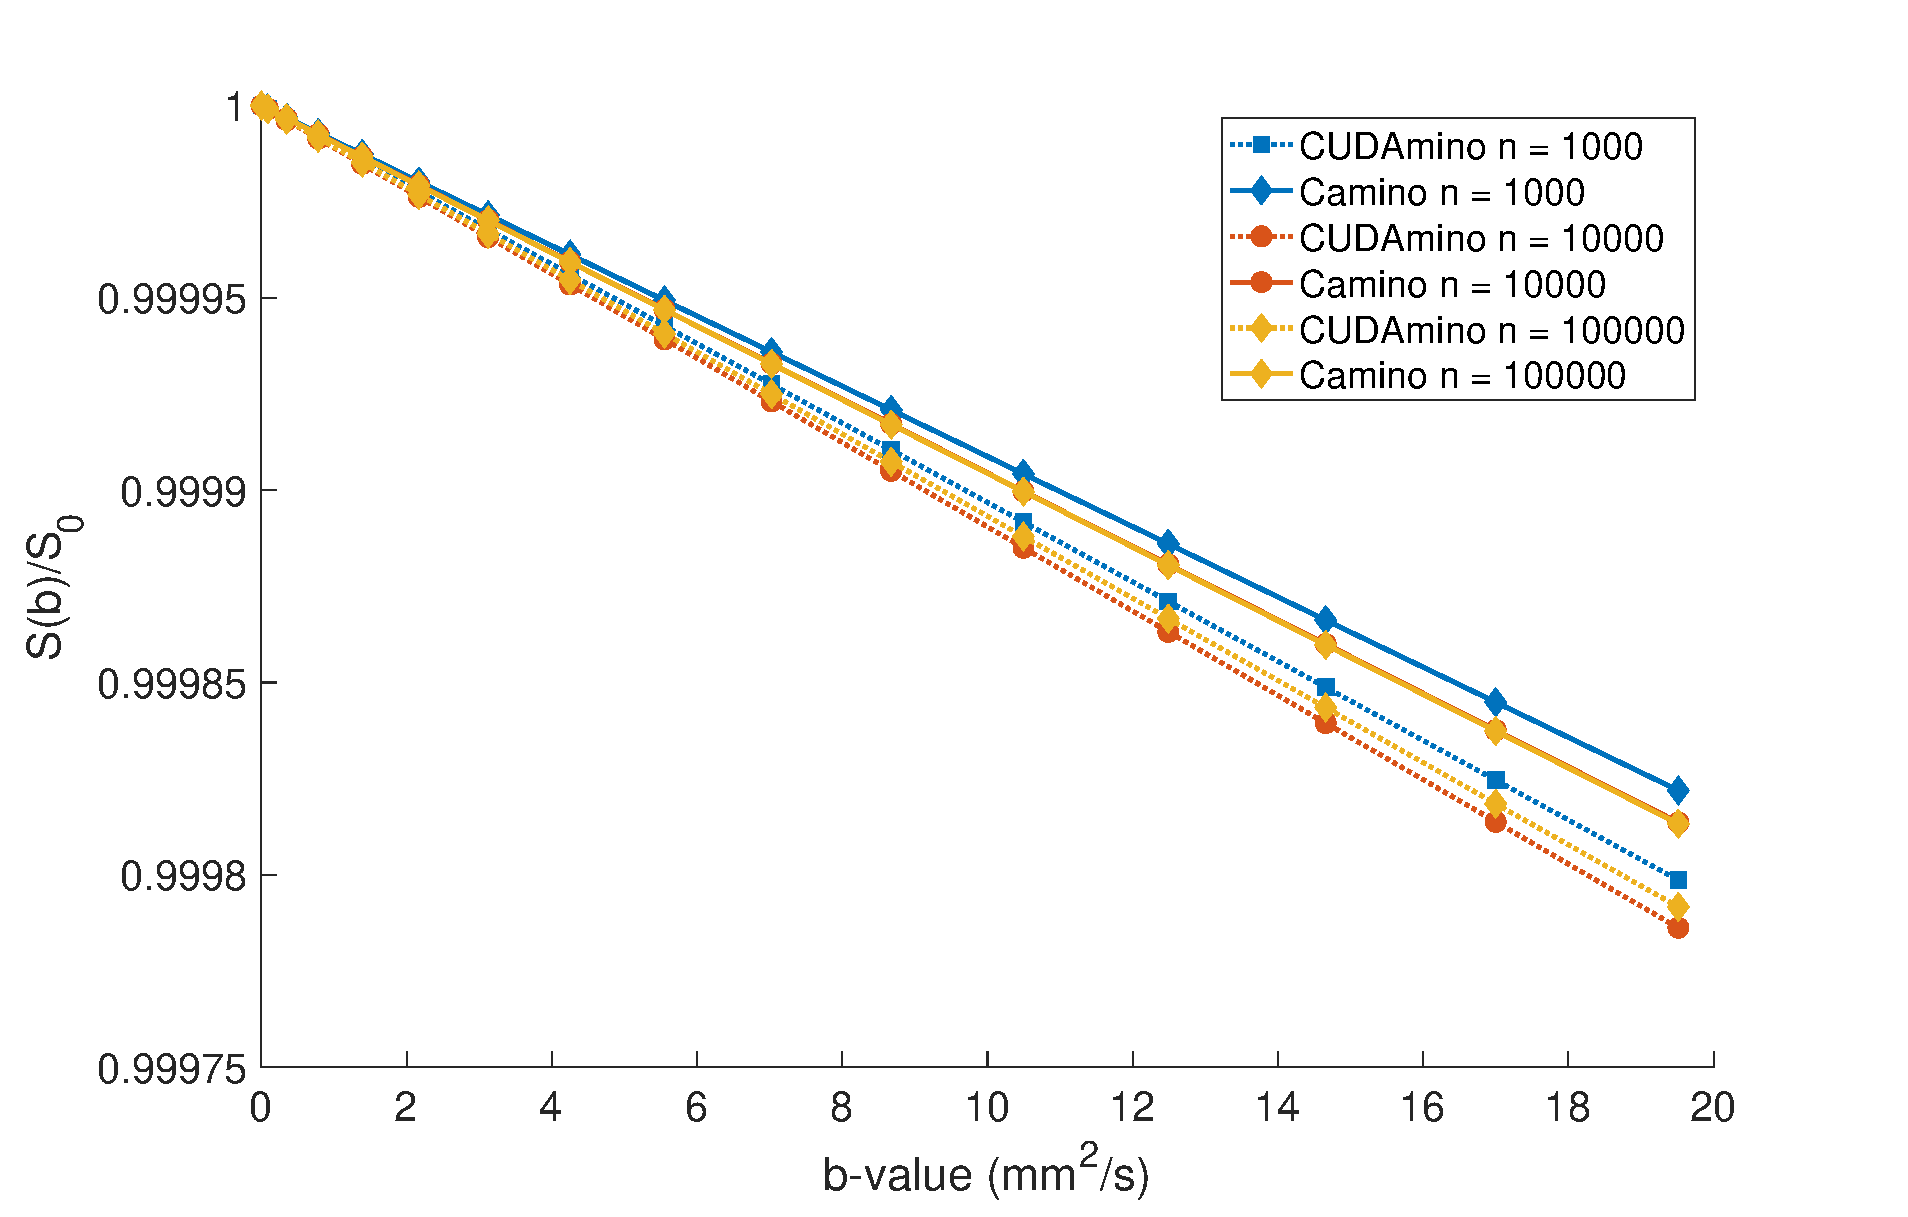
\includegraphics[width=\textwidth]{figures/cudamino/cyl_nspin.eps}
%     \caption{}
%     \label{fig:cyl_nspin_sig}
%   \end{subfigure}
%   ~
%   \begin{subfigure}{0.49\textwidth}
%     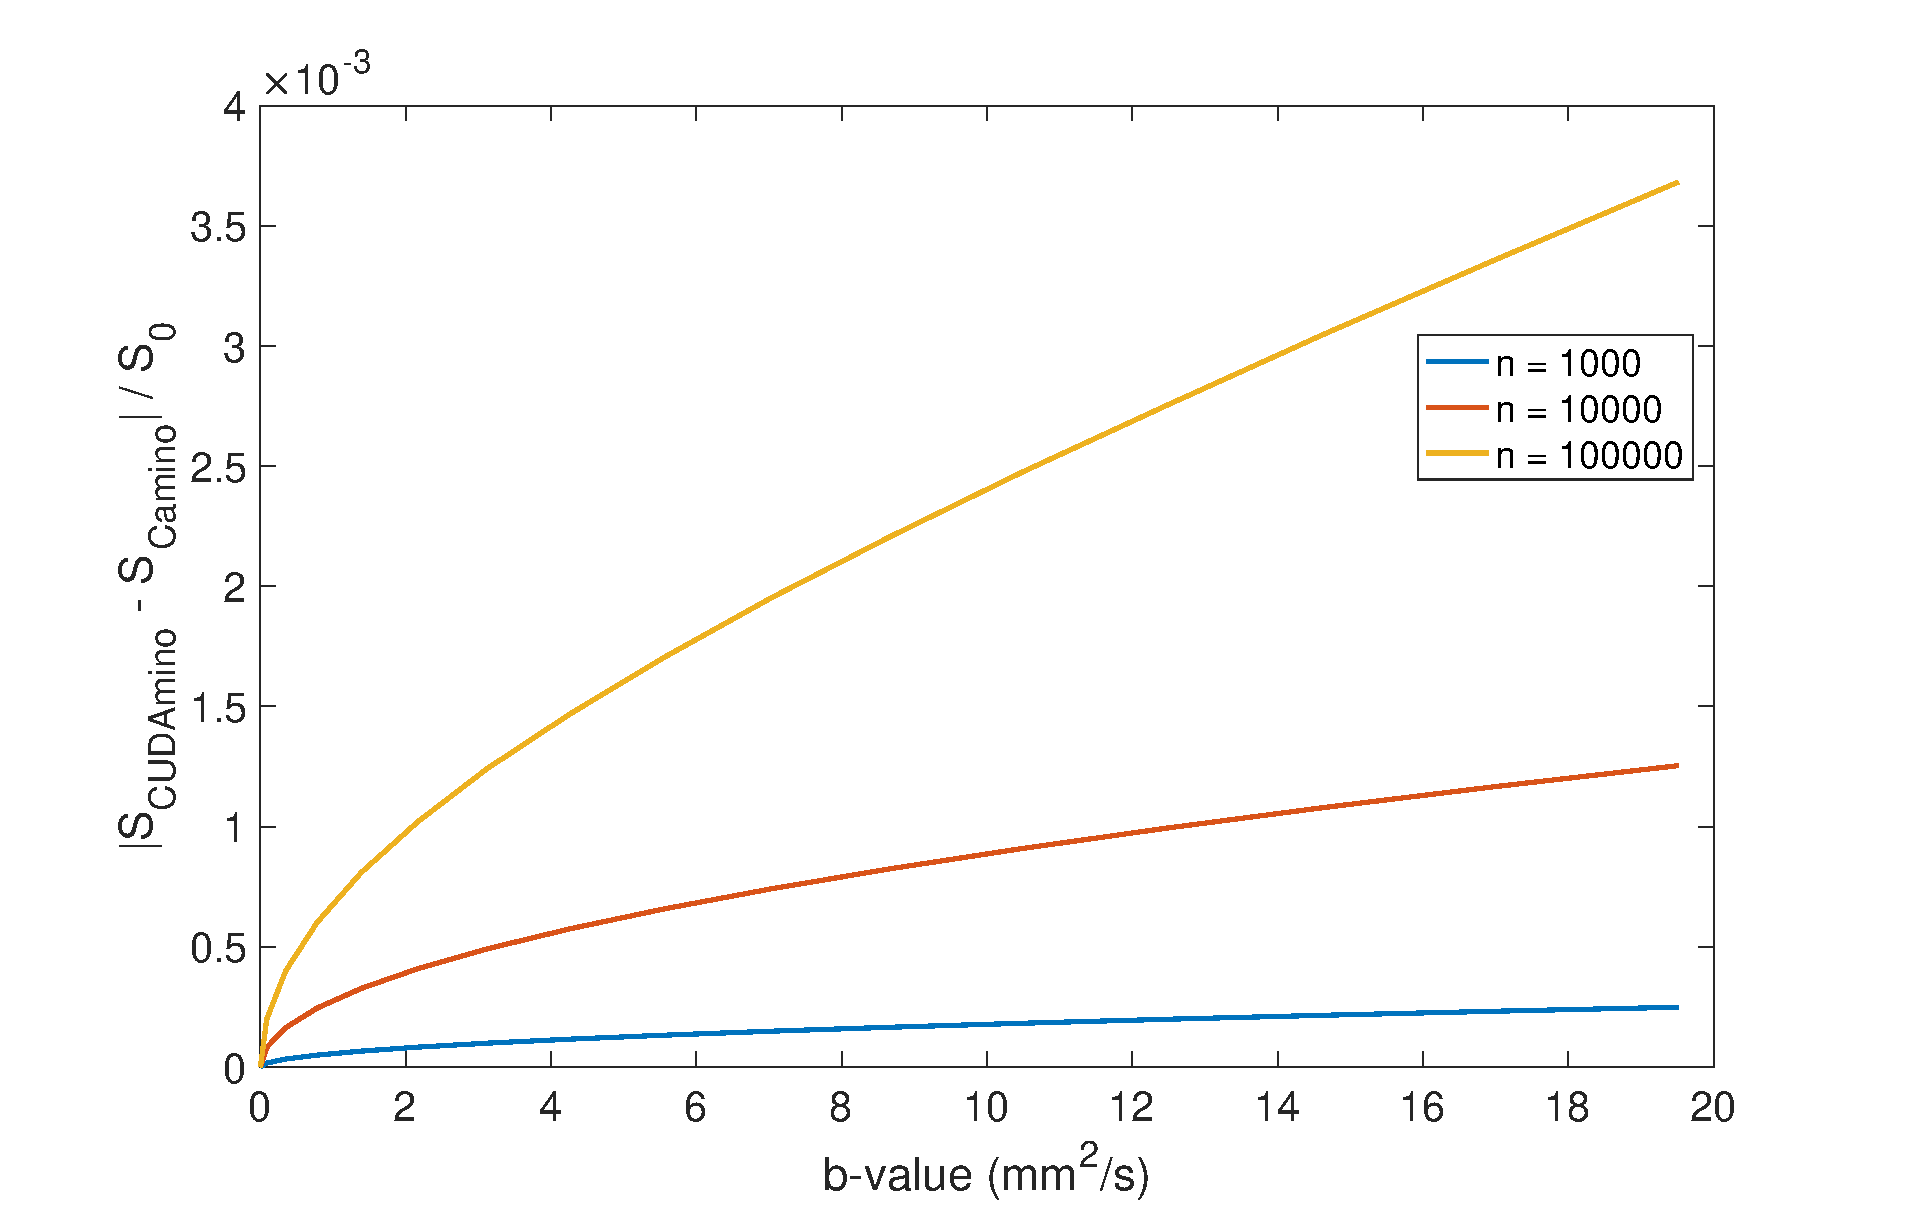
\includegraphics[width=\textwidth]{figures/cudamino/cyl_nspin_diff.eps}
%     \caption{}
%     \label{fig:cyl_nspin_diff}
%   \end{subfigure}
%   \caption{Cylinder tests varying $n$. a) The simulated \ac{dMRI} signals and b) The difference between CUDAmino and Camino signals.}
%   \label{fig:cyl_nspin}
% \end{figure}

\begin{figure}
  \centering
  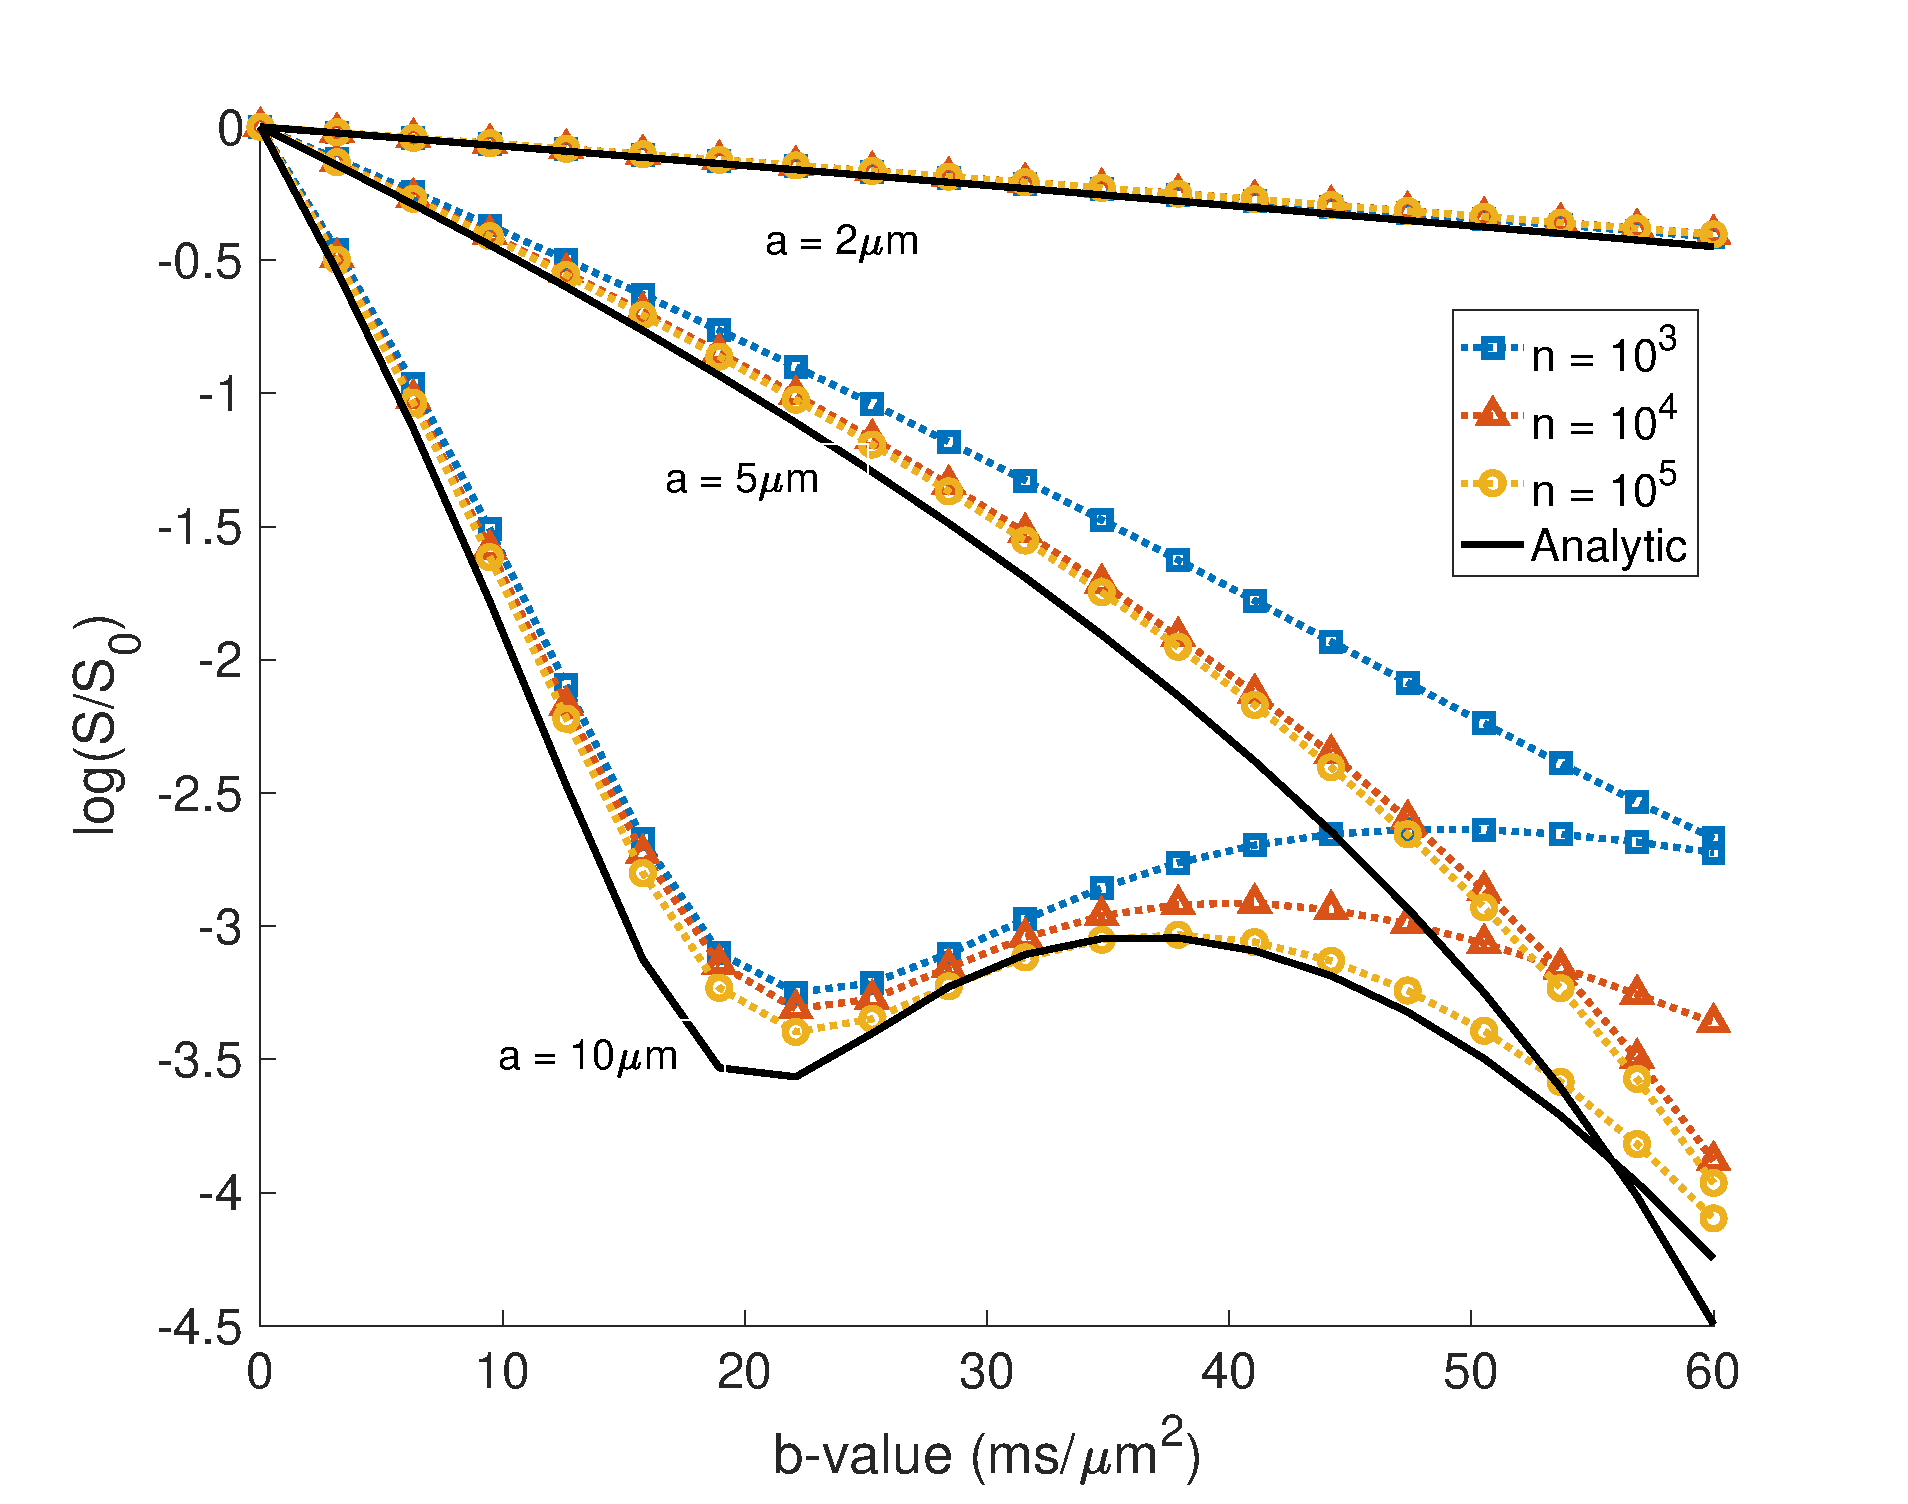
\includegraphics[width=0.8\textwidth]{figures/cudamino/new/cuboid_all_cudamino_nspin_no_1mil.eps}
  \caption[CUDAmino simulations versus analytic solutions for varying $n$.]{CUDAmino simulations (dotted lines) versus analytical solutions (solid black lines) simulations within the cuboid in \Cref{fig:cudamino_cuboid} varying the number of spins, $n$.}
  \label{fig:cuboid_cudamino_nspin}
\end{figure}

% \begin{table}
%   \centering
%   \begin{tabular}{|c|c|c|}
%     \hline
%     $t_{max}$ & Camino Time (s) & CUDAmino Time (s)\\\hline
%     1000 & 317.33& 3.0951\\
%     10000 & 1744.4& 24.547\\
%     50000 & 7333.4& 112.03\\\hline
%   \end{tabular}
%   \caption{Running time comparison of Camino and CUDAmino for experiments with variable $t_{max}$}
%   \label{tab:cyl_tmax_time}
% \end{table}


% \begin{table}
%   \centering
%   \begin{tabular}{|c|c|c|}
%     \hline
%     $n$ & Camino Time (s) & CUDAmino Time (s)\\\hline
%     1000 & 9.0979 &7.0987 \\
%     10000 & 94.402 &7.2175\\
%     100000 & 1124.5 &80.821\\\hline
%   \end{tabular}
%   \caption{Running time comparison of Camino and CUDAmino for experiments with variable $n$}
%   \label{tab:cyl_nspin_time}
% \end{table}


\begin{table}
  \centering
  \begin{tabular}{lcccccc}
    \hline
    %& \multicolumn{6}{c}{Mean Error between simulation and analytic, $|S_{sim} - S_{ana}|$}\\
    & \multicolumn{2}{c}{2$\mu$m} & \multicolumn{2}{c}{5$\mu$m} & \multicolumn{2}{c}{10$\mu$m}\\
    & CUDA & Camino & CUDA & Camino & CUDA & Camino \\\hline
    % Timing & & & & & & \\
    % \hspace{10pt}n=10$^3$ & & & & & & \\
    % \hspace{10pt}n=10$^4$ & & & & & & \\
    % \hspace{10pt}n=10$^5$ & & & & & & \\
    % \hspace{10pt}n=10$^6$ & & & & & & \\\hline
    $t_{max}=10^3$ & 0.0178 & 0.0174 & 0.0198 & 0.0205 & 0.0111 & 0.0076\\
    $t_{max}=10^4$ & 0.0177 & 0.0187 & 0.0173 & 0.0204 & 0.0081 & 0.0088\\
    $t_{max}=5\times10^4$ & 0.0180 & 0.0180 & 0.0210 & 0.0228 & 0.0102 & 0.0074\\\rule{0pt}{3ex}
    $n=10^3$ & 0.0133 & 0.0180 & 0.0626 & 0.0493 & 0.0283 & 0.0087 \\
    $n=10^4$ & 0.0173 & 0.0207 & 0.0242 & 0.0267 & 0.0154 & 0.0109 \\
    $n=10^5$ & 0.0170 & 0.0179 & 0.0198 & 0.0180 & 0.0083 & 0.0076 \\
    %$n=10^6$ & & & & & & \\
    %& & & & & &\\

    \hline
  \end{tabular}
  \caption[Mean error between simulations and analytic results for the cuboid in \Cref{fig:cudamino_cuboid}.]{Mean error between simulations and analytic results for the cuboid in \Cref{fig:cudamino_cuboid}. Values are absolute difference between simulated signal and analytic signal, $|S_{simulated} - S_{analytic}|/S_0$, for the two experiments described in \Cref{sec:cudamino_experiments}. Here CUDAmino is shortened to CUDA to save space. In each case, the value across 5 repeats had insignificant variance.}
  \label{tab:cuboid_results}
\end{table}


\begin{table}
  \centering
  \begin{tabular}{lccc}
    \hline
    &\multicolumn{2}{c}{Running time (s)} & Speedup\\
    & CUDAmino & Camino \\\hline
     $t_{max}=10^3$ & $2.0876 \pm 0.003$ & $241.71 \pm 7.49$ & $115.7\times$\\
    $t_{max}=10^4$ & $19.964 \pm 0.037$ & $2707.3 \pm 27.3$ & $110.5\times$\\
    $t_{max}=5\times10^4$ & $97.739 \pm 0.039$ & $10762 \pm 68.4$ & $111.2\times$\\\rule{0pt}{3ex}
    $n=10^3$ & $0.7797 \pm 0.008$ & $12.059 \pm 0.478$ & $15.46\times$\\
    $n=10^4$ & $1.1385 \pm 0.006$ & $114.82 \pm 0.775$ & $110.9\times$\\
    $n=10^5$ & $10.004 \pm 0.034$ & $1105.1 \pm 11.2$ & $110.5\times$\\\hline
  \end{tabular}
  \caption[Timing results for CUDAmino versus Camino.]{Timing results for CUDAmino versus Camino. For all experiments, CUDAmino shows faster running time with lower variance across runs. The typical speedup is around $100\times$.}
  \label{tab:cuboid_timing}
\end{table}

    

\section{Discussion and Conclusion}
\label{sec:cudamino_discussion}
CUDAmino, as presented here, still has some way to go to fully replicate Camino's diffusion simulations.
There are a number of features lacking, such as permeability and full reflections, however this represents a good first step towards a fully-featured GPU \ac{dMRI} simulator.

As shown in \Cref{fig:cuboid_cudamino_tmax,fig:cuboid_cudamino_nspin}, CUDAmino is able to match the analytic result in a simple substrate. Additionally \Cref{tab:cuboid_results} shows that  the difference between the simulated signals in CUDAmino and Camino is small in the simple scenario presented.
This a promising result as it shows that CUDAmino is able to match analytic results as well as the results of Camino well.
There should be further investigation, however, to investigate how CUDAmino performs in other simple substrates compared to both Camino and analytical results. 

The performance boost that CUDAmino has over Camino, running simulations 15-100$\times$ faster shows the promise that CUDAmino has in making \ac{dMRI} simulations much more efficient.
Most of the simulations had a speedup of over $100\times$, with only the simulations with a small number of spins having the $15\times$ speedup.
For most complex cases, the number of spins required will be significantly higher than 1000, suggesting that in practice, CUDAmino may see typical speedups around $100\times$.

%%% Local Variables:
%%% mode: latex
%%% TeX-master: "../main"
%%% End:
